\documentclass{article}

% 10-703 Style requirement.
% This will set margins, and make the look-and-feel of the document a research paper
\usepackage[final,nonatbib]{nips_2016}

%%Some semiuseful packages
\usepackage[utf8]{inputenc} % allow utf-8 input
\usepackage{amsmath}
\usepackage{amssymb}
\usepackage{fancyhdr}
\usepackage{graphicx}
\usepackage{tikz}
\usepackage{stmaryrd}
\usepackage{enumerate}
\usepackage{fancyvrb}

\usepackage[english]{babel}
\usepackage[backend=bibtex]{biblatex}
\addbibresource{MidtermReport.bib}

\title{10-703 Midterm Report}

\author{
  Roger Liu \\
  \texttt{rogerliu@andrew.cmu.edu} \\
  \And
  Stephen Chen \\
  \texttt{stephen1@andrew.cmu.edu} \\
}
%\date{Due: 28 January 2016}
\begin{document}
\maketitle
\section{Introduction}
In the process of creating video games, a designer’s intentions are not always reflected in the resulting gameplay. A boss monster in an action game might be frustratingly hard, or a particular strategy might allow the player to breeze through a game. To address this, game developers undergo multiple cycles of ``playtesting'' in order to tune their game's difficulty and resulting player experience. This process is expensive and time consuming, as developers must be on hand to observe the playtesting sessions and identify where the game's design fails to create the appropriate amount of challenge. This time investment is greatly exacerbated in Role-Playing Games (RPGs), as the interactions between various character statistics (like health, strength, defense) and gameplay mechanisms can become insurmountably complex, making it difficult for a designer to identify and correct the root of the problem \cite{rpgbalance}. In addition, RPGs usually allow the player to customize their character, specializing their skillsets to deal with different situations as they progress through the game. This is especially difficult to design around, as designers cannot know what tools a player has going into a challenge.

While designers now have many more tools and systems available to make playtesting and data collection easier, there are few systems for automating the difficulty adjustment process. Existing literature mostly focuses on a concept called Dynamic Difficulty Adjustment (DDA). In these systems, the difficulty of the game changes dynamically while a player is playing. For instance, Hunicke and Chapman proposed making reactive (immediate) and proactive (long term) changes to the environment of a first-person shooter game based on the probability of the player’s health dropping to dangerous levels \cite{hunicke2004ai}. Andrade and Corruble dynamically adjusted the difficulty of a fighting game AI by using reinforcement learning to learn optimal state-action values, but then using suboptimal actions based on a ``challenge function'' which scored how well the player was doing \cite{andrade2005challenge}. There are other approaches with adjustment techniques other than RL \cite{spronck2003online,missura2009player}, and different player feedback functions \cite{liu2009dynamic,zook2012temporal}. 

Though these systems are able to change a game's difficulty to provide an appropriate level of challenge to the player, they would not perform well in RPGs. This is because existing DDA algorithms determine difficulty based on a simplified model of game dynamics. For example, in a first-person shooter, the difficulty can be determined just based on how much damage a player is expected to deal vs. how much they are expected to take. These models are acceptable for games where the character statistics are generally simple. In a first-person shooter and fighting game, damage dealt is usually fixed and there are no tools that greatly upset the expected outcome of a situation. However, in an RPG, the player character is expected to grow in strength and gain more tools to work with. Their statistics are no longer fixed, and the interaction between various items and gameplay mechanisms makes it difficult for a DDA with a simple dynamics model to understand when a situation is actually difficult for the player. If such a complex model is known to begin with, then DDA will not even be needed, as developers themselves will understand how to tune the difficulty of a game. In addition, because of the transparent nature of stats in most RPGs, changes made by DDA will be very apparent to the players, which may make them feel cheated out of overcoming the game's challenge. As a result, the difficulty of an RPG is best tuned offline, where the full gameplay model can be simulated many times and without being immediately obvious to the player.

This paper will detail the outline and implementation of a system which will learn to tweak a game environment so that the resulting gameplay difficulty closely matches the intentions of the designers, automating the long iterative process of playtesting.
To do this, we will teach an agent (tentatively known as the ``Dungeon Master'' or DM) to adjust various parameters of an environment (known as the ``Dungeon'') that players will navigate. The DM’s rewards will be to tune the environment so that the game difficulty matches the designer’s intent (i.e. player dies around x times). This problem is tackled through the lens of reinforcement learning. The states are the statistics of the enemies found in the dungeon, and the actions are the ways that the DM can adjusts enemy statistics.

\section{Methods}
In these first two subsections, we discuss the current state of our project implementation. In the last subsection, we discuss the challenges we faced to reach this point.

\subsection{Game Environment}
For this first phase of the project, we settled on having the DM ``solve'' a minimalistic RPG game. In this game, the player character progresses through 2 rooms of a dungeon, fighting one monster in each room. Combat proceeds by having the player and opponent take turns performing actions. The player can choose to either attack or drink one of their limited number of potions to recover their health. The monster always does a basic attack, unless a more powerful special attack is available. The special attack is available every $f$ turns. For our preliminary experiments, if the player is defeated during combat, their death is counted and they are immediately restored to their maximum health with all of their potions. When the monster is defeated, the player ``clears'' the room and moves on to the next room. It is important to note that the players health and potion do not recover when going between rooms.

The parameters that the Dungeon Master are allowed to tune are the damage for each monster's basic and special attack, as well as the frequency ($f$) that they can use their special attack. 

\begin{figure}[h]
	\centering
	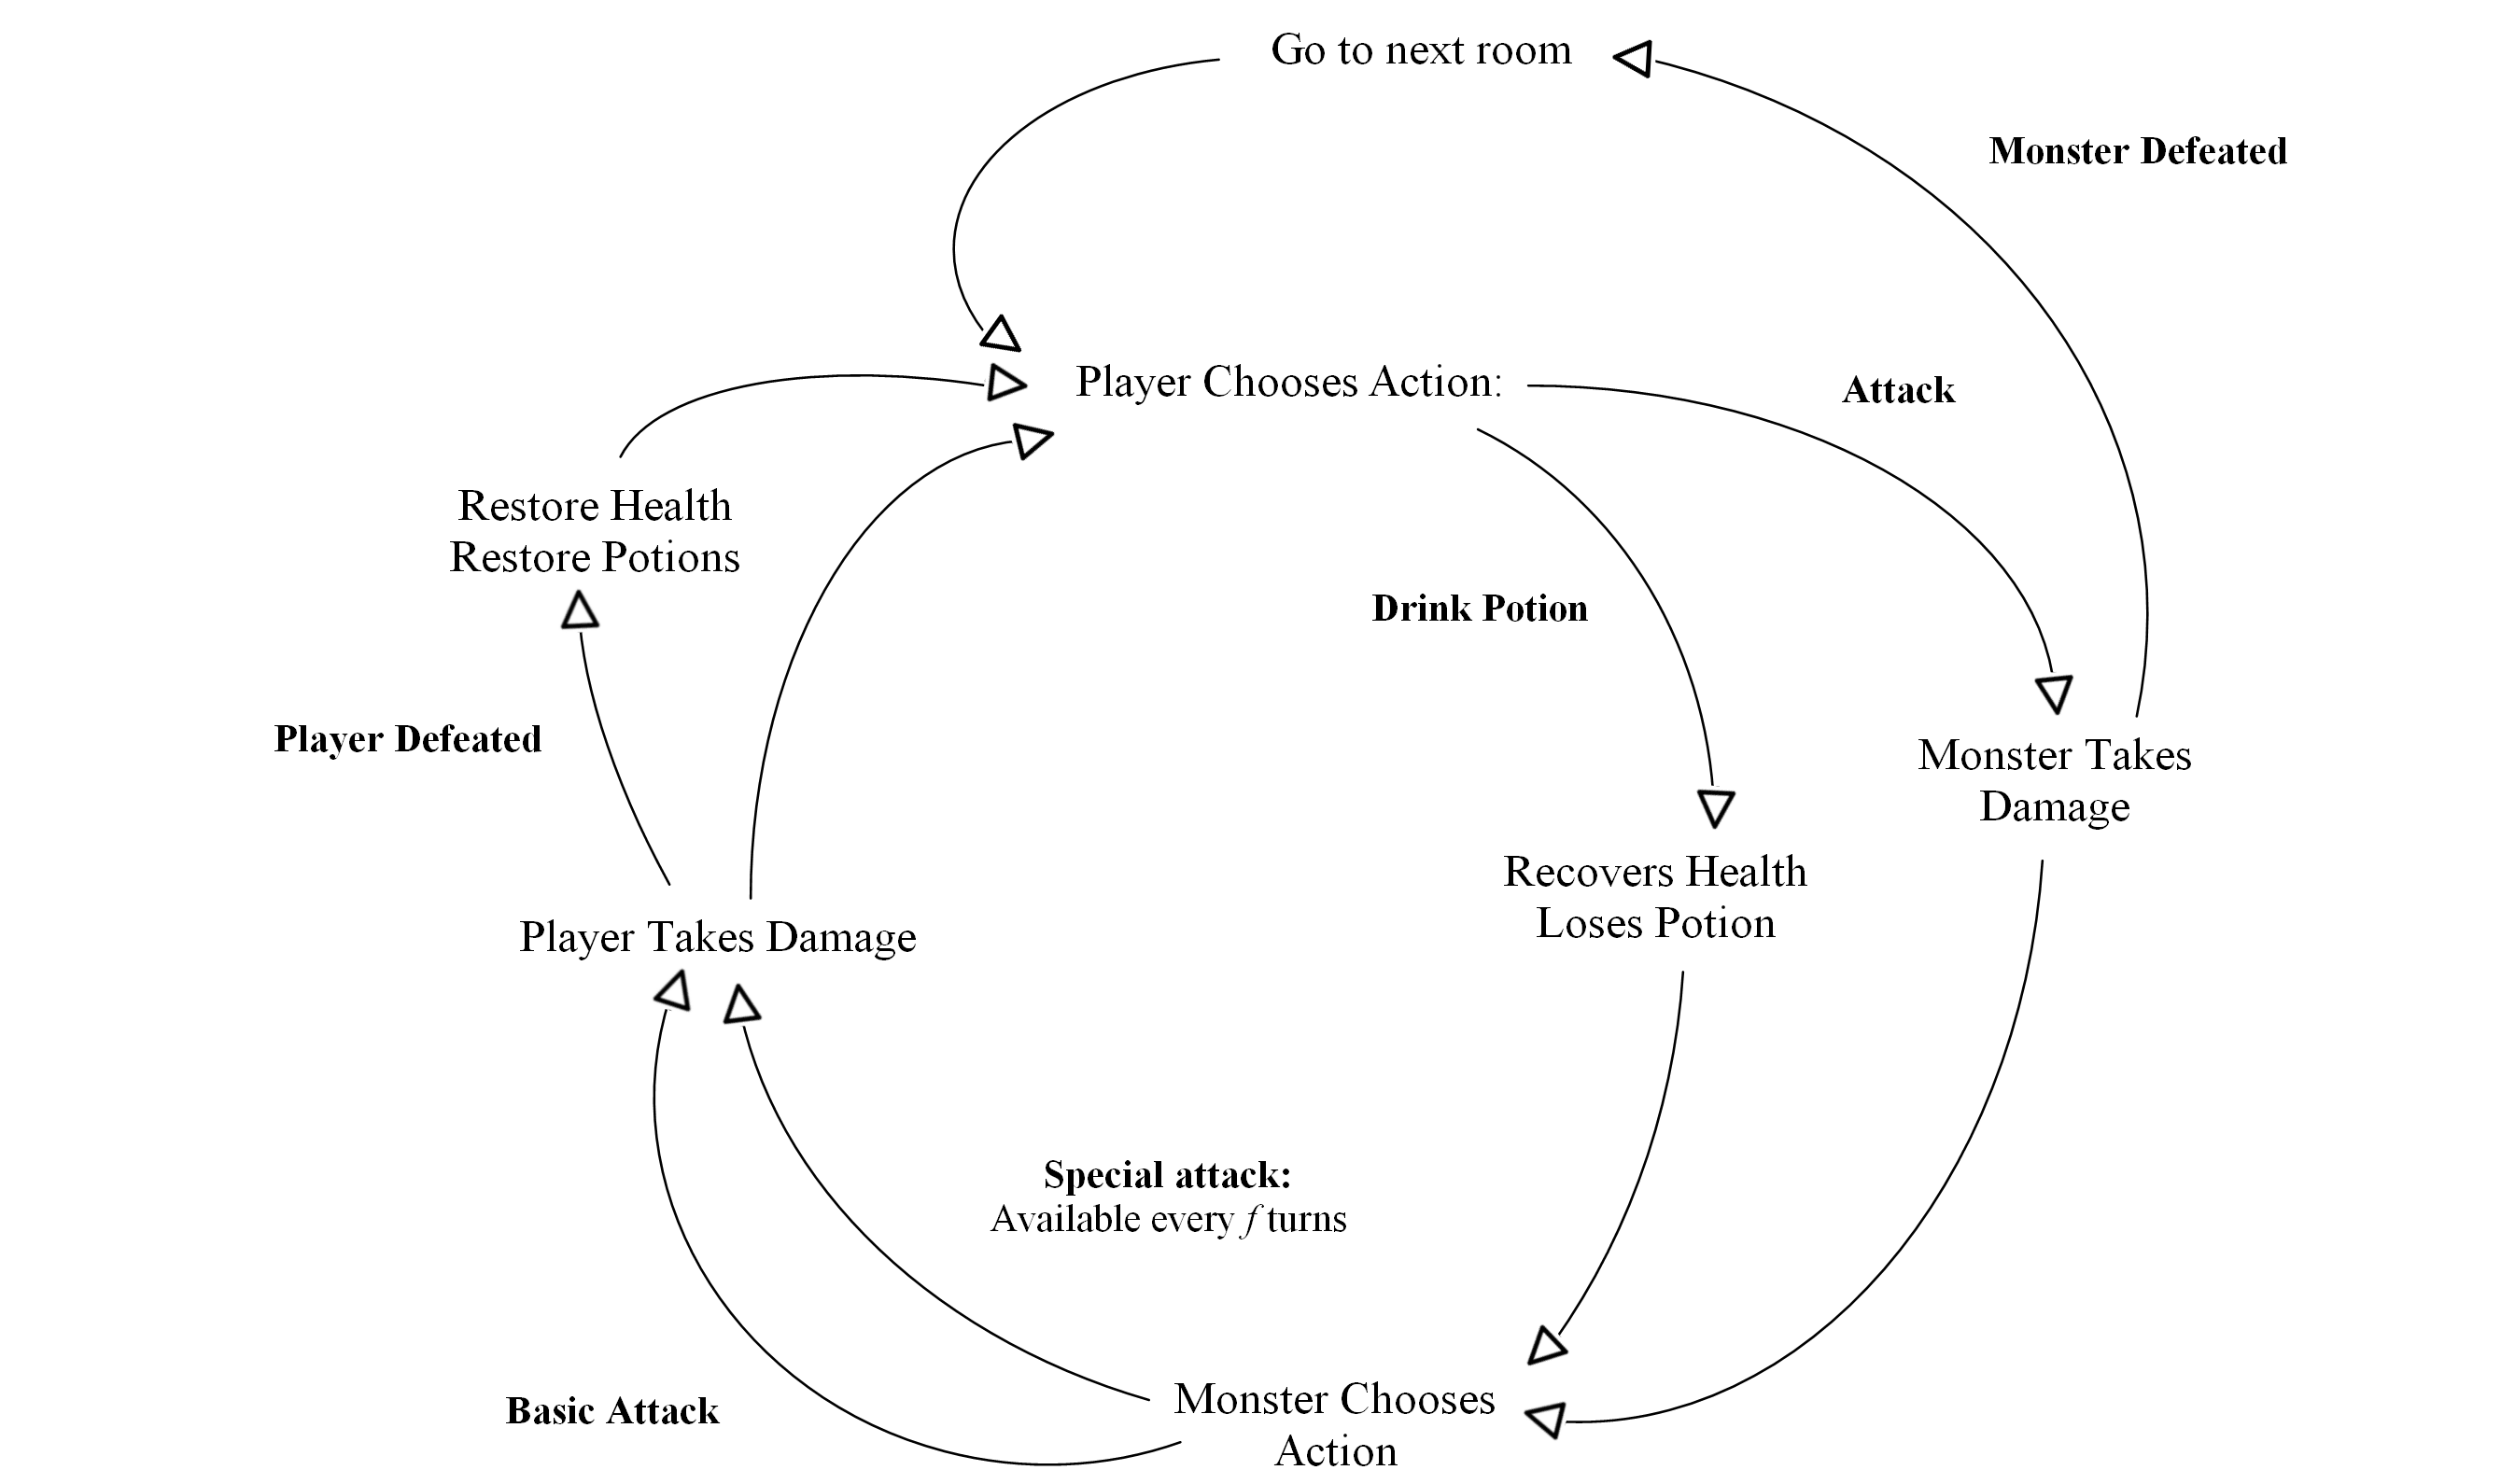
\includegraphics[width=0.6\textwidth]{Gameflow.png}
	\caption{Diagram of Game Flow}
\end{figure}

Once we implemented the framework for the game, we needed a player to play through it. While we would ideally want real people playing through the game, doing so would not be time-efficient or accurately capture a consistent style of play. Thus, for this first phase, we implemented a simple greedy player, who attacks every turn and immediately uses a potion when their health drops below a preset threshold. 

With the game implemented and an agent to automatically play through the game, we can now formulate the problem of adjusting the game as an RL problem.

We designate $x^{(k)}_{i}$ as the $k$th monster's $i$th stat. To be concrete, for monster $k$, $x^{(k)}_{1}$ is the monster's normal attack damage, $x^{(k)}_{2}$ is the monster's special attack damage, and $x^{(k)}_{3}$ is the special frequency $f$. Each statistic has a minimum and maximum value $x_{i, min}, x_{i, max}$. These are specified by the designers, to ensure special attacks are never weaker than normal attacks.

We normalize these stats to [-1, 1] by doing the following:
$$\widetilde{x^{(k)}_{i}} = 2 \frac{x^{(k)}_{i} - x_{i, min}}{x_{i, max} - x_{i, min}} - 1$$

A state $s$ is a configuration of the normalized stats of the monsters in the dungeon, represented as a vector.
$$s = \left\langle \widetilde{x^{(1)}_{1}}, \widetilde{x^{(1)}_{2}}, \widetilde{x^{(1)}_{3}}, \widetilde{x^{(2)}_{1}} \ldots \right\rangle$$

An action is an adjustment of those stats. It is given by:
$$a = \langle m^{(1)}_{1}, d^{(1)}_{1}, m^{(1)}_{2}, d^{(1)}_{2}, m^{(1)}_{3}, d^{(1)}_{3}, m^{(2)}_{1}, \ldots \rangle$$

To apply an adjustment to a stat, we do the following update:
$$x^{(k)}_{i} \leftarrow 1.5^{m^{(k)}_i} \cdot x^{(k)}_{i} + d^{(k)}_i$$
clipping at $x_{i, min}$ or $x_{i, max}$ if necessary. Intuitively, $m$ determines a scaling factor and $d$ is a flat adjustment.

The reward of moving to a state is the euclidean distance between the number of deaths that the player experiences in a playthrough with the new configuration and the designer's intended number of deaths.
\begin{align*}
X_s &= [\text{room 1 deaths}, \text{room 2 deaths}, ...] \\
\mathcal{R}(s, a, s') &= \lVert X_{s'} - target \rVert
\end{align*}


Note here that the states are multi-dimensional continuous variables, and the actions are also multi-dimensional continuous values.


\subsection{Dungeon Master}
We implemented the DM with the TD Actor-Critic method. Specifically we used a variant called Continuous Actor Critic Learning Automaton (CACLA) \cite{van2007reinforcement}. In this variant, we only update the policy weights $\theta$ when the TD error is positive, that is, when the below condition holds
$$\delta_t = R(s_t, a_t, s_{t+1}) + \gamma Q_w(s_{t+1}, a_{t+1}) - Q_w(s_t, a_t)  > 0$$

In addition, our policy weight update is
$$\theta_{t+1} := \theta_{t} + \alpha n \nabla_{\theta_{t}} \log \pi_{\theta_{t}}(s_{t}, a_{t})$$
where $n = \lceil \delta_t / \sqrt{\mathsf{var}_{t}} \rceil$ and $\mathsf{var}_{t}$ is the running average of the variance of $\delta$. Intuitively, the first change means that we only update the actor's policy towards actions that give us positive returns, and we never penalize the policy for giving us bad returns. The second change means that we update the actor's policy more than once when the action that yielded a higher than typical TD error.

The actor and critic are backed by simple linear models. The critic is
$$Q_w(s,a) = w^T \phi(s,a)$$
where $\phi$ just flattens the input vectors together.

The actor is given by
$$\mu_{\theta}(s) = \theta_w s + \theta_b \qquad a \sim \mathcal{N}(\mu(s), \sigma^2)$$ 
where $\theta_w$ is a matrix of weights, $\theta_b, \mu, a, \sigma$ are vectors, and $a$ is the actual action taken. $\sigma$ here represents ``Gaussian exploration.'' Higher values of $\sigma$ will cause the actor to explore actions further away than the one given by $\mu$. Values for each component in $\sigma$ are given by the game, as the game understands what's a reasonable exploration range for each action.

The $\sigma$ values are scheduled to linearly decay to $0.01$ of their original value over the first million steps. This effectively reduces the exploration, and implies a stronger belief in the actor's chosen action. This is partly to mimic a linearly decreasing $\epsilon$ in $\epsilon$-greedy, but also to ensure that the actor is taking smaller steps once the critic has a good approximation of the state space.

The Dungeon Master is not made aware of each stat's minimum and maximum value when picking its continuous actions. As according to the CACLA paper, this should not be an issue.

\subsection{Progression of the DM}
Initially, the actor model did not have the bias weights $\theta_b$, and the actions we picked were just a vector of scaling factors (rather than exponents):
$$a = \langle m^{(1)}_{1}, m^{(1)}_{2}, m^{(1)}_{3}, m^{(2)}_{1}, \ldots \rangle$$
with an adjustment application like such
$$x^{(k)}_{i} \leftarrow m^{(k)}_i \cdot x^{(k)}_{i}$$

Recall that our DM is allowed to pick any value in the real numbers as its action, and it is not limited by adjusted stat's minimum and maximum value. The issue is that this action set has a ``sweet spot'' around $[0.3, 3.0]$ (30\% to 300\% of the original stat). However, by nature of the linear model, the actor would often pick scaling factors like $-2$ or $5$, which are not very reasonable (i.e. it wanted $-200\%$ of the original stat). Because it was often unable to locate the ``sweet spot'', our DM would often bounce between very extreme actions: dropping all monster stats to their minimum or raising all monster stats to their maximum.

We initially combated this with a lower learning rate. This stabilized the learning for a while, but after a thousand steps the actor would be stuck in a minima. A few hundred thousand steps later, the Q-values would suddenly start dropping to negative infinity.

Our next attempt was by augmenting the actor models with a bias vector $\theta_b$, in hopes that the DM would learn a bias around $1$ to keep its actions in sweet spot. In addition, we greatly lowered the Gaussian exploration variance $\sigma$. While this succeeded in stabilizing the system, it also resulted in heavily reducing the rate of exploration and actually did not solve our local minima and divergence issues.

Reconsidering the problem, it became apparent that the odd ``sweet spot'' was too much of an issue. The difference between an action of $1.0 \to 0.5$ meant that a stat would be scaled in half, but the difference from $1.0 \to 1.5$ meant that it was scaled up by less than half. This unevenness was no doubt an issue. We thus considered that it would be best if the $m_i$ were centered around 0. We thus changed the adjustment equation, so that the agent output's $m_i$ served as the exponential of a scaling term. That is something like $x_i \leftarrow 2^{m_i}x_i$. Semantically, this works better because a negative value scales the stat to a lower value, and a positive value scales the stat to a higher value. This significantly improved our performance, and we noted that the monster stats were no longer being dropped to minimum or raised to maximum values.

The flat adjustment $d^{(m)}_i$  was later added to give the DM more control over adjusting the stat.

\newpage
\section{Preliminary Results}

Our most notable improvement came when we changed the DM's action set to be an exponential scaler of a monster's stats rather than a linear one. 

Here we show the results of the agent before and after the change

\subsection{Metrics for Linear Scaling}
\begin{figure}[h]
	\begin{minipage}{0.5 \textwidth}
		\centering
		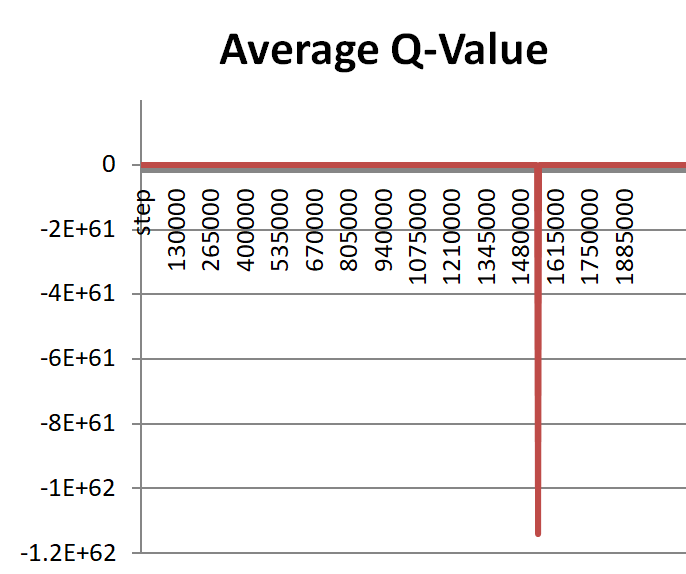
\includegraphics[width=0.9\textwidth]{AverageQBad.png}
		\caption{Linear Scaling Q-Value}
	\end{minipage}
	\begin{minipage}{0.5 \textwidth}
		\centering
		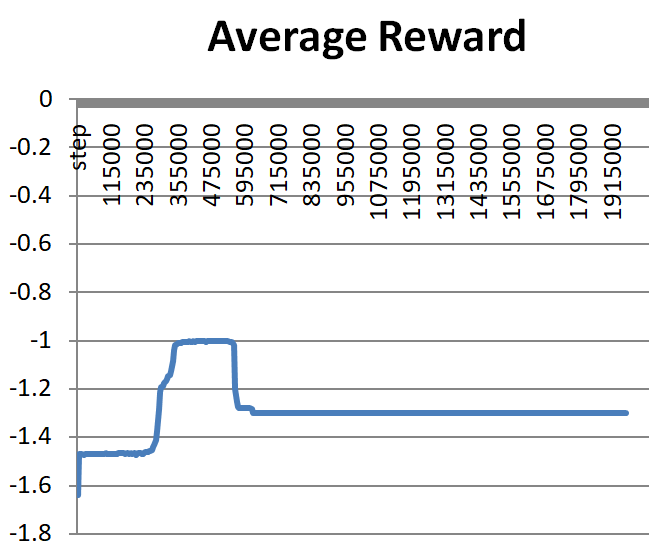
\includegraphics[width=0.9\textwidth]{AverageRewardBad.png}
		\caption{Linear Scaling Average Reward}
	\end{minipage}
\end{figure}

Commentary: These graphs show what happened when we were using the $x^{(k)}_{i} \leftarrow m^{(k)}_i \cdot x^{(k)}_{i}$ stat adjustment equation. Though the agent initially seemed to improve in average reward (Figure 3), it soon fell into a rut where it failed to improve the dungeon at all. During this time, it pushes the dungeons parameters to the extremes (max or min stats for everything). Note the sharp dip in Average Q-Value graph (Figure 2), and note the scale. It is at the sharp dip that the DM's started to pick scaling factors like 40 and -60, and the Q-Values started diverging to negative infinity.

\newpage
\subsection{Metrics for Exponential Scaling}
\begin{figure}[h]
	\begin{minipage}{0.5 \textwidth}
		\centering
		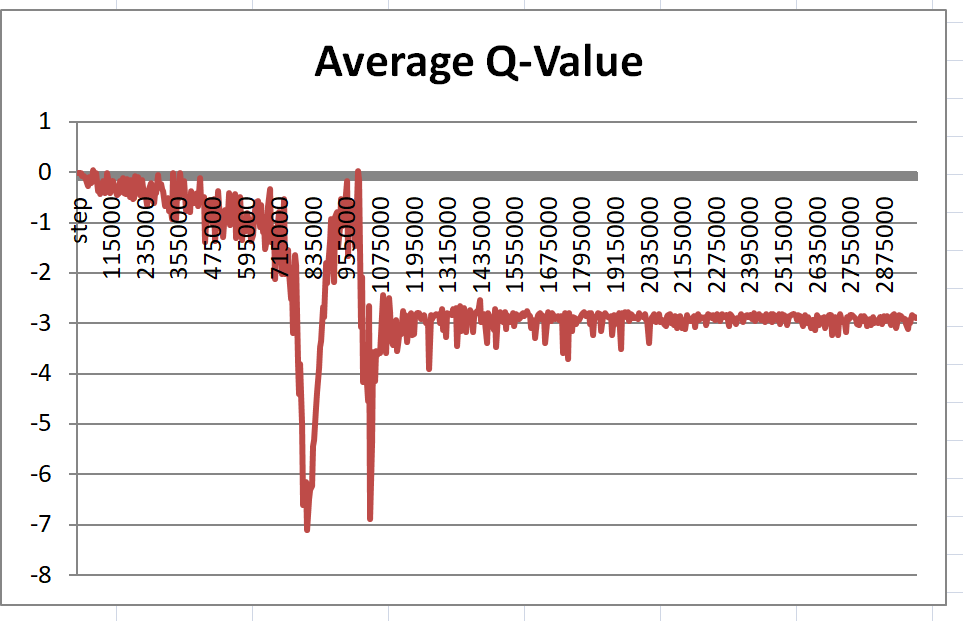
\includegraphics[width=0.9\textwidth]{AverageQ.png}
		\caption{Exponential Scaling Q-Value}
	\end{minipage}
	\begin{minipage}{0.5 \textwidth}
		\centering
		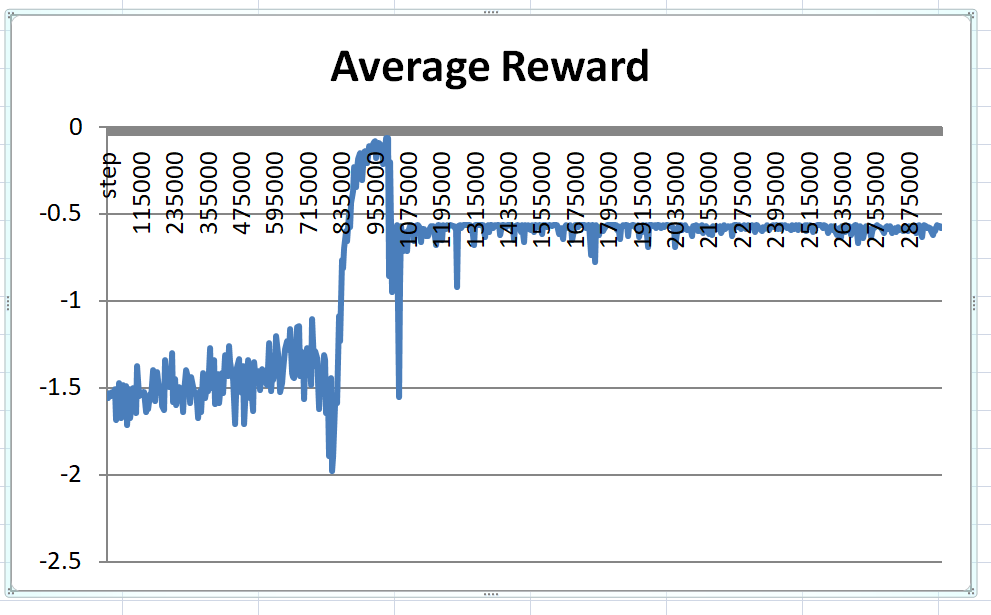
\includegraphics[width=0.9\textwidth]{AverageReward.png}
		\caption{Exponential Scaling Average Reward}
	\end{minipage}
\end{figure}
\begin{figure}[h]
	\begin{minipage}{0.5 \textwidth}
		\centering
		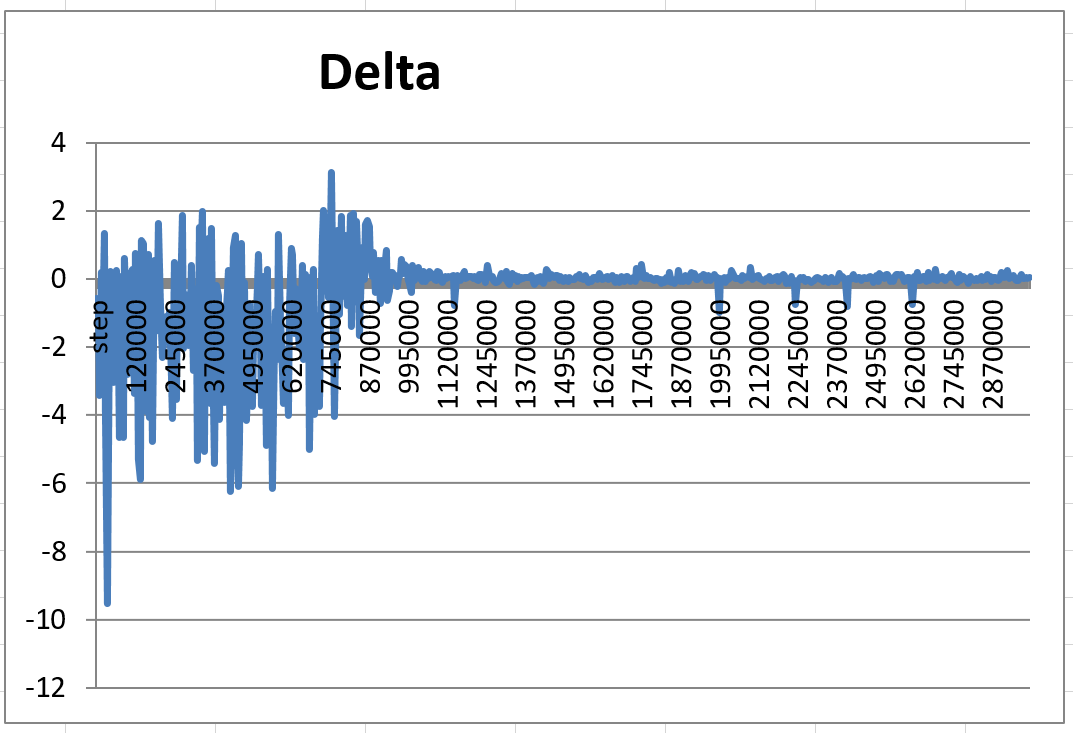
\includegraphics[width=0.9\textwidth]{Delta.png}
		\caption{Exponential Scaling - TD Error $\delta$}
	\end{minipage}
	\begin{minipage}{0.5 \textwidth}
		\centering
		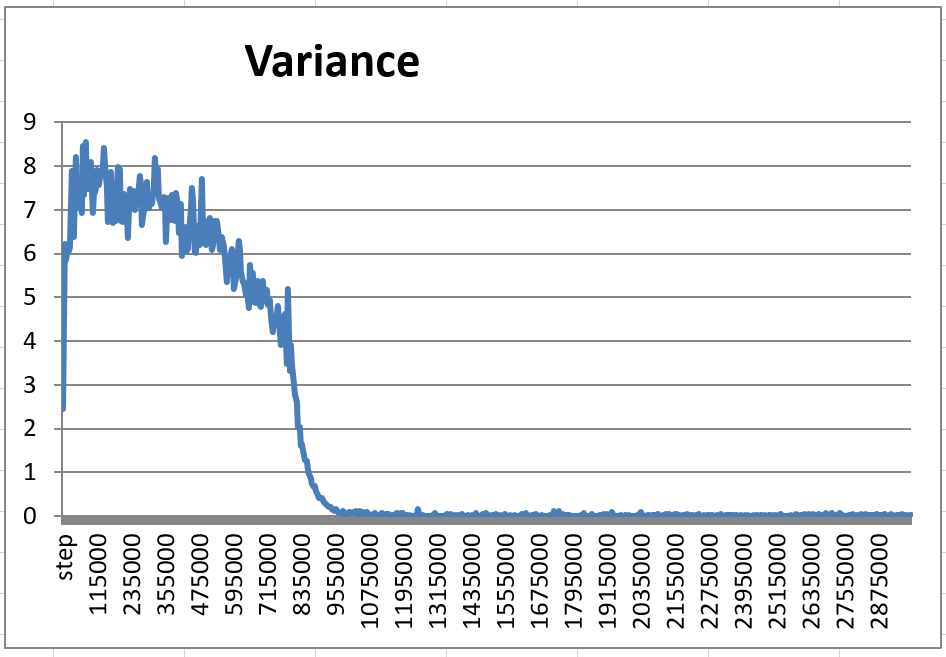
\includegraphics[width=0.9\textwidth]{Variance.png}
		\caption{Exponential Scaling - Variance of TD Error $\delta$}
	\end{minipage}
\end{figure}

Commentary: These are the results attained after switching to the $x^{(k)}_{i} \leftarrow 1.5^{m^{(k)}_i} \cdot x^{(k)}_{i} + d^{(k)}_i$ update rule. When we implemented an exponential rather than a linear scaling factor, we got a much better behaved agent. It no longer diverges and even reaches a point where the dungeon actually matches the target number of deaths set out by the designers. As it keeps running it eventually fits to something that is outside that perfect balance, but the values it settles on perform much better than the other attempts. To circumvent this problem of falling out of the perfect goal state, we can tweak the agent to stop immediately once it reaches the goal.

\section{Final Plan}
\quad \quad We plan to expand the game into a fuller version called \textit{Minimal RPG}. We aim to have more rooms, more monsters per room, and more stats for both the player and monsters to increase the complexity. The monsters will also drop potions, and if time permits we will try to get the player to level up to introduce more complexity. In addition, we will be trying to implement a smarter player algorithm than the one we described (potentailly using another reinformacement algorithm), likely one that will introduce more stochasticity to the DM's reward function. Finally, we aim to create some human-playable version of the game, so that we can evaluate if the DM has appropriately tuned the difficulty of the dungeon.

\printbibliography

\end{document}
